\section{Problema 3: Heurística Constructiva Golosa}

\subsection{Descripción de la problemática}
En este caso se nos pide colaborar en la asignación de aulas con diversos recursos a un conjunto de materias (con un horario establecido e invariable) que necesitarían hacer uso de ellos durante el dictado de clase.\\
Como en este caso nos interesa distinguir las aulas de acuerdo a sus recursos, le asignaremos a cada una un color (suponiendo que no hay dos aulas que cuenten con idénticos recursos) y uniremos con aristas aquellas que se han querido reservar para horarios cuya intersección no es vacía.\\
Dicho esto, nuestra tarea consiste en generar un algoritmo que implemente una heurística cuyo objetivo sea encontrar alguna forma de colorear los nodos, minimizando en la medida de lo posible la cantidad de conflictos (entendidos estos como instancias que impiden que el coloreo generado sea válido, es decir, que verifique que para toda arista L que a sus nodos adyacentes se les haya asignado distinto color.) 


\subsection{Resolución propuesta y justificación}

\subsection{Análisis de la complejidad}


\subsection{Código fuente}
% A continuación se incluyen las partes más relevantes del código.
% La clase \emph{Lector.java} se encarga de tomar los datos del archivo de entrada y procesarlos para construir el grafo.
% \lstinputlisting[name=pp, numbers=left, frame=lines, firstline=51, lastline=129]{../src/ej2/src/Lector.java}
% La clase \emph{Solucion.java} contiene los métodos que calculan el camino mínimo del grafo entre los dos puntos señalados.
% \lstinputlisting[name=pp, numbers=left, frame=lines, firstline=14, lastline=76]{../src/ej2/src/Solucion.java}

\subsection{Experimentación}



% \begin{figure}[H]
%    \begin{center}
%  	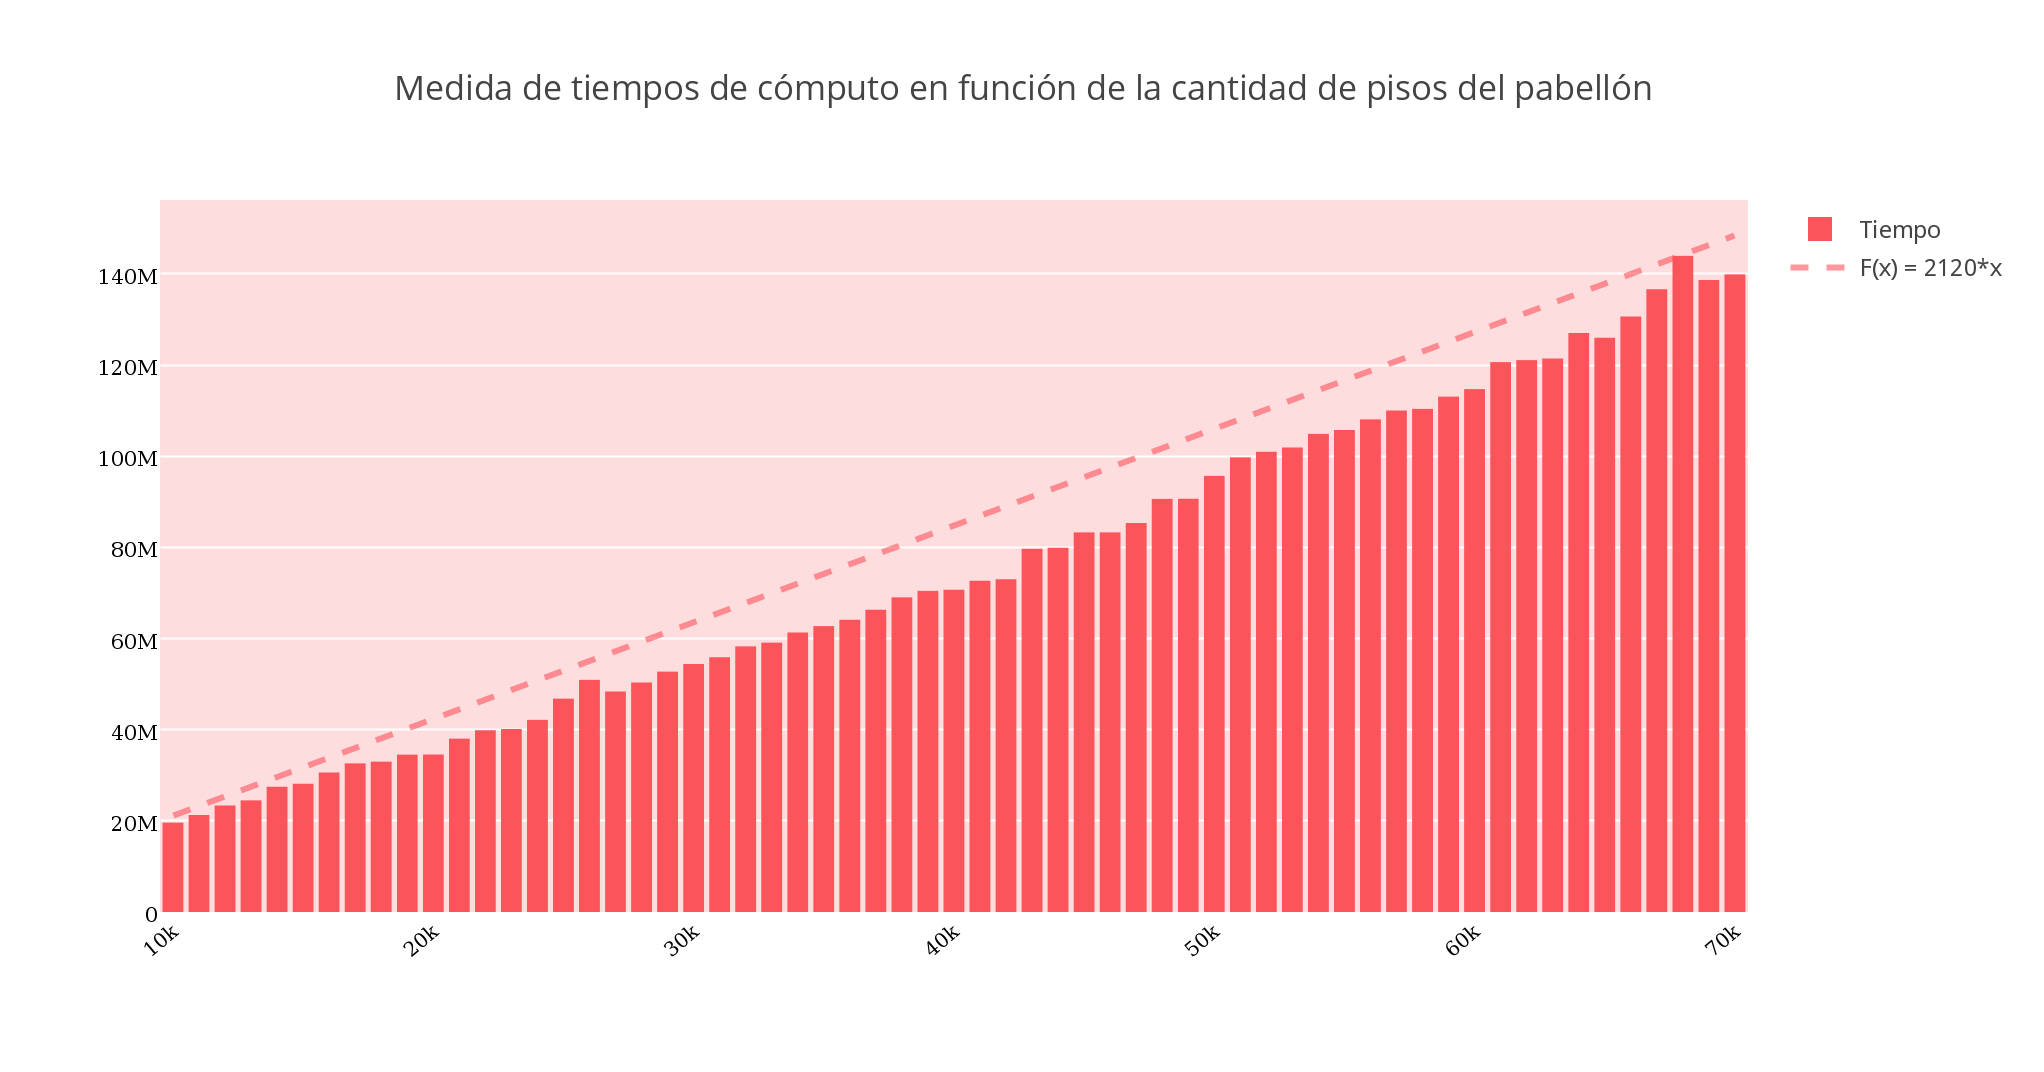
\includegraphics[width=18cm]{imagenes/ej2/f(pisos).png}
% 	\caption{Medición de tiempos en función de la cantidad de pisos}
% 	\label{pisos}
%    \end{center}
%  \end{figure}

 

\subsubsection{Peor caso}

\subsubsection{Mejor caso}



\newpage
